\chapter{Motivación e introducción}

En este capítulo se explica la aquitectura de una FPGA en comparación con otros circuitos integrados digitales. Además se mencionan los campos de aplicación más 
importantes. Aquí también, se detallan los distintos niveles de síntesis automática (síntesis funcional, RT-lógica y física). 
Por último se hace mención a varios fabricantes de FPGAs con sus respectivos dispositivos y a las herramientas software de desarrollo, 
dando más importancia a las de Xilinx y algunas plataformas de propósito académico del fabricante Xilinx.

\section{Sistemas basados en dispositivos FPGAs} 

Las FPGAs (\textit{Field Programmable Gate Arrays}), son dispositivos semiconductores basados en matrices de bloques lógicos configurables
(\textbf{CLB}) que están conectados mediante interconexiones programables (Figura \ref{arqFPGA}) \cite{fpga_xilinx}. 

\begin{figure}[H]
    \centering
    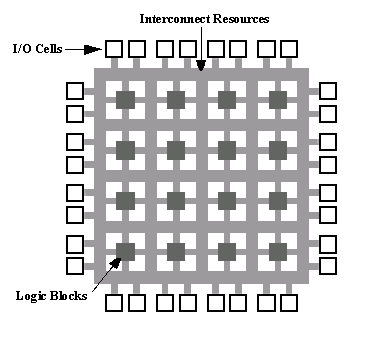
\includegraphics[width = 0.5\textwidth]{imagenes/arqFPGA.png}
    \caption{\textit{Arquitectura de una FPGA \cite{arquitectura}}}\label{arqFPGA}
\end{figure}

Los bloques lógicos configurables en las FPGAs basadas en celdas SRAM incluyen LUTs (\textit{tablas de consulta}), flip-flops y 
multiplexores de entrada y salida. Una LUT almacena una lista de salidas lógicas para cualquier combinación de 
entradas.

Estas FPGAs pueden ser reprogramadas para  algún trabajo específico o para cambiar los requisitos de funcionalidad después de su 
fabricación. Algunas pueden ser programadas una sola vez mientras que otras pueden ser reprogramadas una y otra vez. A estos 
dispositivos que son programados una única vez son referidos como \textbf{OTP} (\textit{one-time programmable}).

\textit{Field Programmable}, se refiere al hecho de que su programación se hace ``\textit{en el campo}'' a diferencia de otros dispositivos 
que su funcionalidad está programada por el fabricante \cite{maxfield1}.

Las tres principales tecnologías usadas para programar una FPGA son: \textbf{Antifusible}, \textbf{SRAM}, \textbf{Flash}

La tecnología \textbf{Antifusible} es una tecnología no reprogramable, por lo tanto son \textit{OTP}. Son dispositivos que permiten establecer 
conexiones entre distintas capas de metal. No es volátil y además la conexión entre los bloques lógicos tiene un retardo muy reducido, por lo 
que el rendimiento es alto. Sin embargo, las FPGAs antifusibles necesitan un proceso de fabricación específico y por lo tanto es caro. 

La tecnología \textbf{SRAM} es una tecnología reprogramable con una reprogramación muy rápida. Sin embargo, las FPGAs basadas en esta tecnología 
son volátiles, lo que significa que los datos de configuración del dispositivo se perderán cuando se desconecte la energía. 

La tecnología \textbf{Flash} es reprogramable como la \textbf{SRAM} y además es no volátil como la \textbf{Antifusible}. Utiliza menos potencia 
que la \textbf{Antifusible} con un proceso de fabricación basado en transistores de puerta flotante.

Hay muchos tipos diferentes de circuitos integrados digitales, entre los que destacamos \textbf{PLDs} (\textit{Programmable Logic Devices}), 
\textbf{ASICs} (\textit{Application-Specific Integrated circuits}), \textbf{ASSPs} (\textit{Application-Specific Standard Parts}) y \textbf{FPGAs}.

Los \textbf{PLDs} son dispositivos con una arquitectura interna predeterminada por el fabricante. También son configurables ``in situ'' con tecnologías basadas en fusibles, 
antifusibles y EPROM o EEPROM. En comparación a las \textbf{FPGAs}, contiene un número limitado de puertas lógicas 
y las funciones que se suelen implementar son más pequeñas y simples.

Por otro lado los \textbf{ASICs} y los \textbf{ASSPs} contienen cientos de millones de puertas lógicas y se usan para crear grandes y complejas 
funciones. Ambos están basados en los mismos procesos de diseño y tecnologías y pueden ser usados por millones de usuarios y compañias. La 
única diferencia es que un \textbf{ASIC} está diseñado y fabricado para una aplicación en concreto, mientras que un \textbf{ASSP} lo está 
para un dominio de aplicaciones.

Así, las \textbf{FPGAs} se encuentran entre los \textbf{PLDs} y los \textbf{ASICs} porque su funcionalidad puede ser diseñada en el campo como 
los \textbf{PLDs}, pero pueden contener millones de puertas lógicas y ser usadas para implementar funciones complejas que previamente sólo 
podían ser realizadas usando \textbf{ASICs}. 

El coste de un diseño de \textbf{FPGA} es mucho menor que el de uno de un \textbf{ASIC}. Al mismo tiempo, los cambios de diseño implementados 
son más fáciles en \textbf{FPGAs} y el tiempo de comercialización es más rápido \cite{maxfield2}.

Las FPGAs \textbf{SoC}(\textit{System-on-chip}), que es un circuito integrado que tiene todos los componentes necesarios para un sistema electrónico.
Además de la lógica genérica configurable incluyen empotrados en hardware uno o varios procesadores, memoria DDR, interfaces para buses 
estándar, interfaces de comunicaciones, e incluso unidades de procesamiento gráfico. Tienen una gran capacidad de procesamiento para 
adaptarse a diferentes aplicaciones. Una FPGA SoC de bajo costo y consumo se puede utilizar en aplicaciones como tarjetas de procesamiento de 
vídeo. Sin embargo, hay otros FPGA SoCs que se utilizan en aplicaciones de alto rendimiento en comunicaciones o computación de alto rendimiento.

A mediados del año 1980 llegaron las FPGAs, que eran usadas para implementar lógicas simples, máquinas de estados con una complejidad media 
y tareas de procesamiento de datos. A principios de los 90s, el mercado en el que se vendían se extendió al área de las telecomunicaciones 
debido a que el tamaño y sofisticación de las mismas empezaron a crecer. A finales de los 90s, el uso de las FPGAs en aplicaciones de consumo 
e industriales tuvo un enorme crecimiento.

Las FPGAs a menudo son utilizadas para crear prototipos de diseños ASIC o para tener un plataforma hardware donde verificar la implementación 
física de nuevos algoritmos \cite{maxfield1}. 

Actualmente se pueden encontrar FPGAs de alto rendimiento con millones de puertas. Algunos de estos dispositivos tienen núcleos de 
microprocesador integrados, dispositivos de entrada-salida de alta velocidad y similares. El resultado es que actualmente las FPGAs pueden ser 
usadas para implementar sistemas en distintos ámbitos como por ejemplo:

\begin{itemize}
    \item \textbf{Aeroespacial y defensa} 
    \item \textbf{Emulación y Prototipado}
    \item \textbf{Audio} 
    \item \textbf{Automoción} 
    \item \textbf{Broadcast} 
    \item \textbf{Electrónica de consumo} 
    \item \textbf{Centro de procesamiento de datos} 
    \item \textbf{Computación de alto rendimiento} 
    \item \textbf{Industria} 
    \item \textbf{Medicina} 
    \item \textbf{Comunicaciones}
    \item \textbf{Inteligencia Artificial}
    \item \textbf{Procesamiento de imágenes}
    \item \textbf{Seguridad}
\end{itemize}

\section{Niveles de síntesis automática}
La metodología es un concepto abstracto referido a un conjunto de procesos que relacionan entre sí los niveles de complejidad y abstracción 
(\textit{funcional o de comportamiento}, \textit{arquitectural o transferencia de registros}, \textit{lógico o de puertas} y 
\textit{físico}), por los que pasa el diseño de un circuito \cite{teres1997vhdl}.

Los niveles de abstracción son:

\begin{itemize}
    \item \textbf{Funcional o de comportamiento}: Se indica el comportamiento del circuito como una relación funcional entre las entradas 
    y salidas, sin tener en cuenta la implementación.
    \item \textbf{Arquitectural o de transferencia de registros}: Se realiza una partición de bloques funcionales y se planifican las 
    operaciones que se van a realizar en cada ciclo de reloj. 
    \item \textbf{Lógico o de puertas}: Componentes expresados como ecuaciones lógicas o puertas y elementos de una biblioteca genérica o 
    específica de una tecnología.
    \item \textbf{Físico}
\end{itemize}

En general, establecer una metodología o flujo de diseño consiste en definir las distintas etapas por los que pasarán los distintos niveles 
de abstracción y fijar cómo pasar de unos niveles de abstracción a otros usando procesos manuales o automáticos de:

\begin{itemize}
    \item \textbf{Síntesis}: Pasar descripciones de un nivel de abstracción a otro con mayor detalle (por ejemplo, de una descripción RT a 
    puertas, o de puertas a física).
    \item \textbf{Análisis}: Extraer información de un descripción para verificar prestaciones o para validar restricciones en un nivel 
    de abstracción superior.
    \item \textbf{Verificación / Simulación}: Validar las descripciones de cada etapa.
\end{itemize}

Para la realización del flujo de diseño, se puede seguir una evolución ``\textit{Top-Down}'' empezando por la idea de la implementación 
o se puede seguir una evolución ``\textit{Bottom-Up}'' comenzando por el nivel físico hasta llegar al funcional.

El diseño ``\textit{Top-Down}'' consiste en partir de una idea con un alto nivel de abstracción y partiendo de ella, implementarla y si es necesario 
incrementar el nivel de detalle. Con este diseño se consigue una mayor adecuación a las especificaciones y requisitos.

El diseño ``\textit{Bottom-Up}'' consiste en la descripción del circuito con componentes que se pueden agrupar en módulos hasta llegar al 
sistema completo que se desea. Este diseño está condicionado por los componentes del diseño que están disponibles.

Los lenguajes de descripción de hardware (\textit{HDL}) son lenguajes de alto nivel, similares a los de programación (C, PASCAL, ADA, ...), con una sintaxis y semántica 
definidas para facilitar el modelado y descripción de circuitos electrónicos, desde las celdas de base de un ASIC hasta sistemas completos, pudiéndose 
realizar estas descripciones a distintos niveles de abstracción, precisión y estilos de modelado.
Los HDL modelan el comportamiento de un componente de cara a su simulación, aunque también se utilizan para describir el diseño de un circuito para
su implementación a través de etapas de síntesis validadas vía simulación.

Los primeros lenguajes que fueron estándar IEEE son \textbf{VDHL} y \textbf{Verilog}. Estos lenguajes se han ido desarrollando y consolidando durante bastante tiempo con el 
fin de dar soporte a las distintas etapas y niveles de abstracción del proceso de diseño. El lenguaje \textbf{VHDL} aparece con el fin de disponer una herramienta 
estándar e independiente para la especificación (modelado y/o descripción) y documentación de los sistemas electrónicos a lo largo de todo su ciclo de vida. 
Tiene una sintaxis más compleja y estricta, que reduce la posibilidad de errores. 
El lenguaje \textbf{Verilog} nace como un lenguaje de modelado ligado a un entorno de simulación, llegando a convertirse en un estándar ``de facto'' a nivel
industrial. Tiene una sintexis más simple, parecida a C y múltiples versiones \cite{teres1997vhdl}.

Una de las características principales de un lenguaje de descripción hardware es que a partir de una descripción se puede generar un 
circuito físico. La síntesis es el paso de un nivel de descripción a uno de nivel inferior.

La síntesis física consiste en la ubicación, es decir, decidir dónde colocar todos elementos lógicos, y en el enrutamiento, en el que se 
decide cómo se interconectan los elementos en la FPGA.

La síntesis RT-lógica es un proceso en el se crea un diseño RTL (\textit{Register-Transfer Level}), que es una abstracción del diseño 
en el que se modela el circuito digital, y luego esa representación RTL es convertida a un conjunto de registros y ecuaciones 
booleanas equivalentes. 

La principal diferencia entre síntesis RT y síntesis de alto nivel es que la primera parte de una descripción en la que de forma 
explícita se especifican las operaciones que deben realizarse en cada ciclo de reloj, mientras que la planificación de operaciones 
en ciclos de reloj se realiza de forma automática en la segunda.

La síntesis de alto nivel une hardware y software de manera que los diseñadores hardware pueden trabajar con un alto nivel de abstracción 
y los desarrolladores software pueden acelerar partes computacionalmente complejas de sus algoritmos en una FPGA. 

El uso de una metodología de diseño de síntesis de alto nivel permite desarrollar algoritmos semejantes a los que se emplea en 
programación software, validar el correcto funcionamiento de un diseño de forma más rápida que con lenguajes de descripción 
hardware tradicionales y crear implementaciones hardware de alto rendimiento.

\section{Plataformas de desarrollo} 

En este apartado se exponen los principales fabricantes de FPGAs, destacando a Xilinx, herramientas software de desarrollo  de diversos fabricantes y 
plataformas de propósito académico.

\subsection{Principales fabricantes de FPGAs}

Actualmente hay muchas empresas que fabrican FPGAs, pero las más importantes son \textit{Xilinx}, \textit{Intel}, \textit{Microchip Technology} y
\textit{Lattice Semiconductor} \cite{mercado}. 

\textit{Microchip Technology} adquirió \textit{Atmel} y \textit{Microsemi}. Este fabricante proporciona dispositivos que abarcan el rango medio 
y alto, ofreciendo tres familias principales de FPGAs \cite{microchip}:

\begin{enumerate}
    \item \textbf{FPGA IGLOO2} - son FPGAS de gama media y baja, con tecnología flash dedicadas a funciones de propósito general.
    \item \textbf{FPGA SoC SmartFusion2} - están basados en los dispoditivos IGLOO2 incluyendo un procesador ARM-Cortex.
    \item \textbf{FPGA SoC PolarFire} - son dispositivos de alto rendimiento, basados en tecnología flash, de costo optimizado, implementados en tecnología de procesos de 28nm.
\end{enumerate}

Una de las características diferenciales de este fabricante son las FPGAs que son tolerantes a altas radiaciones y están dirigidos a entornos como el espacio. Destacan \textit{RTG4} y 
\textit{RT ProASIC3} basadas en tecnología flash, \textit{RTAX} y \textit{RTSX-SU} basadas en tecnología antifusible.

\textit{Lattice Semiconductor} proporciona también dispositivos de rango bajo y medio y ofrece cuatro principales familias de FPGAs \cite{lattice}:

\begin{enumerate}
    \item \textbf{iCE} - son dispositivos basados en tencología SRAM con memoria no volátil (NVM). 
    \item \textbf{CrossLink y CrossLinkPlus} - CrossLink está basado en tecnología SRAM mientras que CrossLinkPlus en tecnología flash, con una memoria no volátil (NVM). 
    Están diseñadas preferentemente para aplicaciones de vídeo.
    \item \textbf{MachXO} - estos dispositivos están basados en tecnología SRAM, con memoria flash. Diseñados especialmente para aplicaciones seguridad y control.
    \item \textbf{ECP} - son dispositivos basados en SRAM y destinados a aplicaciones de uso general.
\end{enumerate}

El principal competidor de \textit{Xilinx} es \textit{Intel}, que adquirió \textit{Altera}, comercializa FPGAs basadas en tecnología SRAM de gama alta 
(\textit{Agilex}, \textit{Stratix}), gama media (\textit{Arria}) y  gama baja (\textit{Cyclone}). Algunas de estas familias incluyen FPGAs SoCs que 
integran arquitecturas multicore basadas en procesadores ARM (Agilex y Stratix 10 con ARM  Cortex-A53; Arria 10, Arria V y Cyclone V con ARM Cortex-A9). 

Xilinx tiene bastante variedad de FPGAs en cuanto a coste y rendimiento. Actualmente, la serie \textit{Virtex}, la serie \textit{Zynq-7000 SoC}, 
la serie \textit{Zynq UltraScale$+$ MPSoC} y la serie \textit{Zynq UltraScale$+$ RFSoC} ocupan el mercado de gama alta, la serie \textit{Kintex} y 
la serie \textit{Zynq UltraScale$+$ MPSoC} de gama media y la serie \textit{Artix} de gama baja junto con la \textit{Spartan} 
que ha sido retirada del mercado.

La serie \textit{Virtex} se basa en \textbf{CLBs}, donde cada uno de ellos equivale a varias puertas \textit{ASIC}. Cada CLB 
se compone de sectores que son distintos para cada uno de los miembros de esta familia. Además de lógica configurable, se incluyen módulos ``hard-core'' 
para la memoria, bloques \textbf{DSP} (Procesador de señales digitales), controladores PCI Express, entre otros. En esta familia encontramos: \textit{Virtex-II}, 
\textit{Virtex-4}, \textit{Virtex-5}, \textit{Virtex-6}, \textit{Virtex-7}, \textit{Virtex-7 (3D)} y \textit{Virtex UltraScale}.

La serie \textit{Artix} se basa en la arquitectura unificada de la serie \textit{Virtex}. Esta serie está diseñada para aplicaciones con rendimiento de bajo consumo.

La serie \textit{Kintex} se caracteriza por consumir menos energía que la serie \textit{Virtex}, incluyendo alto rendimiento.

\subsection{Herrramientas software de desarrollo}
Dependendiendo de la síntesis que queramos realizar podemos encontrar distintos software:

\begin{itemize}
    \item \textbf{Herramientas de síntesis RT-lógica}:
        \begin{itemize}
            \item \textit{Synplify Pro}, \textit{Synplify Premier} (\textit{Synopsys}) \cite{synopsis}
            \item \textit{Precision RTL Plus}, \textit{LeonardoSpectrum} (\textit{Mentor Graphics}) \cite{mentor}
            \item \textit{Quartus} (\textit{Altera}) \cite{quartus}
            \item \textit{Vivado} (\textit{Xilinx}) \cite{vivado1}
        \end{itemize}
    \item \textbf{Herramientas de síntesis de alto nivel}:
        \begin{itemize}
            \item \textit{Vitis Unified Software Platform} (\textit{Xilinx}) \cite{vitis}
            \item \textit{Synphony C Compiler} (\textit{Synopsys})
            \item \textit{Impulse coDeveloper} (\textit{Impulse C})
            \item \textit{Vivado High Level Synthesis} (\textit{Xilinx})
            \item \textit{SDSoc} (\textit{Xilinx})
            \item \textit{SDAccel} (\textit{Xilinx})
        \end{itemize}
\end{itemize}

En cuanto a la síntesis de alto nivel, Altera apostó inicialmente por basarla en descripciones OpenCL multiplataforma, actualmente con la 
herramienta Intel FPGA SDK for OpenCL Software Technology \cite{intelsdk}. Más recientmente, saca al mercado una herramienta basada en 
descripciones ANSI C++, denominada Intel HLS compiler \cite{intelhls}.

Dentro de los fabricantes de FPGAs, Xilinx ha liderado el desarrollo de herramientas de síntesis de alto nivel basadas en descripciones 
C/C++ (\textit{Vivado HLS}  fué comercializado en 2013) y de entornos de desarrollo orientados a la aceleración de aplicaciones C/C++/OpenCL 
buscando facilitar su uso a ingenieros software, sin necesidad de tener un perfil hardware más específico (SDSoC, SDAccel y actualmente Vitis).

La última herramienta comercializada por Xilinx, \textit{Vitis} \cite{vitis} es un entorno de desarrollo de aplicaciones que sustituye a las herramientas 
\textit{SDSoc} y \textit{SDAccel} que permite utilizar tanto FPGAs en tarjetas aceleradoras on premise y en la nube, como FPGAs con procesadores 
empotrados. Incorpora una herramienta de síntesis de alto nivel (\textbf{Vitis HLS}) que pretende reducir las diferencias entre escribir 
funciones para su ejecución software o para su implementación hardware. Y se dispone incluso de bibliotecas con funciones prediseñadas 
para diferentes dominios de aplicación (inteligencia artificial, visión, etc.).

\subsection{Plataformas de propósito académico}

Las plataformas de desarrollo con propósito académico que comercializa Xilinx son \cite{students} \cite{support}:

\begin{itemize}
    \item \textbf{7-series} - \textit{Basys3}, \textit{Nexys4/DDR}
    \item \textbf{Zynq} - \textit{ZedBoard}, \textit{ZYBO}, \textit{PYNQ-Z1}, \textit{PYNQ-Z2}
    \item \textbf{Spartan} - \textit{Atlys}, \textit{Nexys3}
    \item \textbf{Virtex} - \textit{Genesys}, \textit{XUPV5}
\end{itemize}

Algunas de estas FPGAs están introducidas en las tarjetas vendidas por la empresa \textbf{Digilent}, que 
diseña, fabrica y distribuye herramientas de diseño electrónico, haciendo más accesible esta tecnología 
a estudiantes. Se asocia principalmente con Xilinx para crear plataformas usadas para el aprendizaje. Entre todas las 
tarjetas que ofrece esta empresa encontramos las tarjetas \textit{Basys 3}, que es una placa de desarrollo exclusiva para Vivado y sobretodo para 
estudiantes y principiantes en la tecnología FPGA \cite{basys}, y \textit{Arty A7}, especial para gente que ha estado más en contacto con esta tecnología \cite{arty}, 
con arquitectura FPGA Xilinx Artix-7, \textit{PYNQ-Z1}, está diseñada para usarse con PYNQ, un nuevo marco de código abierto que permite a los programadores explotar las 
capacidades de Xilinx Zynq APSoC sin tener que diseñar circuitos lógicos programables. En cambio, el APSoC se programa usando Python y el código se desarrolla y prueba 
directamente en el PYNQ-Z1 \cite{pynq1}, \textit{Zybo Z7} (Ver apartado 1.1.2) y \textit{ZedBoard}, placa de desarrollo de bajo costo con el que se puede crear 
un diseño basado en Linux, Android, Windows u otro sistema operativo \cite{zed}, con arquitectura Zynq-7000 SoC, \textit{Basys 2}, es una plataforma de diseño e 
implementación de circuitos para que los estudiantes estudien la construcción de circuitos digitales reales \cite{basys2}, con una FPGA Spartan-3E, 
\textit{Arty S7}, es el miembro más reciente de la familia Arty para fabricantes y aficionados y ofrece mejor tamaño y rendimiento \cite{artys7}, 
con una Spartan-7, \textit{Anvyl}, es una plataforma de desarrollo de circuitos digitales completa y lista como plataforma de entrenamiento \cite{Anvyl}, 
con una Spartan-6 y \textit{Genesys 2}, es una plataforma de desarrollo de circuitos digitales avanzada, de alto rendimiento \cite{genesys}, con una Kintex-7. 

\section{Estructura de la memoria} 

Al comienzo de este proyecto se realiza un resumen donde se describe el contenido de este proyecto de una forma resumida además 
de mostrar las palabras clave. Y a continuación se encuentra el mismo resumen y palabras clave, pero en inglés.

Una vez realizada la motivación e introducción en el Capítulo 1 de la memoria que contiene el concepto del que partimos, el concepto de FPGA, 
explicando su arquitectura y haciendo comparaciones con otros circuitos integrados digitales y se mencionan los campos de aplicación más 
importantes. Además, en este capítulo se detallan los distintos niveles de síntesis automática (síntesis funcional, RT-lógica y física). 
Por último se hace mención a varios fabricantes de FPGAs con sus respectivos dispositivos, a las herramientas software de desarrollo 
dando más importancia a las de Xilinx y algunas plataformas de propósito académico del fabricante Xilinx.

En el capítulo 2 se muestran los objetivos del trabajo planteados conseguir durante la realización de este TFG.

Mejor haz referencia al apartado de Materiales (en general) y muy importante al de Metodología. Date cuenta de que la mayor parte del tiempo la has invertido en aprenderla.

Como resolución del trabajo se encuentra el capítulo 3 que está dividido en 4 subapartados, el de Materiales en el que se describe las características de la Familia 
Zynq-7000, así como las de la tarjeta usada (ZYBO) y la descripción de la plataforma utilizada para poder realizar proyectos. También está el subapartado de la Metodología, 
donde se explican las distintas etapas del flujo de diseño y en los otros dos subapartados se explican los módulos hardware que fomarán parte de la plataforma de prácticas, 
un procesador, una memoria RAM, un módulo de generación de reloj y un controlador VGA, y se realizan un par de casos prácticos haciendo uso de los módulos explicados en las secciones anteriores. 

El capítulo 4 contiene las conclusiones y vías futuras del proyecto y del aprendizaje realizado.

A continuación se presenta un anexo que describe de forma práctica el flujo de diseño de sistemas meiante síntesis RT como toma de contacto de la herramienta Vivado 
y la tarjeta Zybo.

Por último está la bibliografía que contiene la información relevante de los libros, artículos y páginas visitadas para la realización del proyecto.